\subsection{Double negative metamaterial}

\begin{frame}{Double negative metamaterial}
    \begin{columns}
        \column{0.5\textwidth}

        \begin{figure}
            \centering
            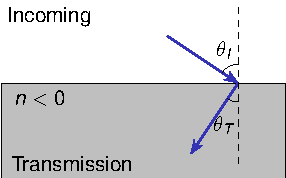
\includegraphics[width=\textwidth]{Figures/LH_Snell.pdf}
            \caption{Refraction with negative index.}
            \label{fig:LH_snell}
        \end{figure}
        \column{0.5\textwidth}
        \vspace{-8mm}
        \begin{figure}
            \centering
            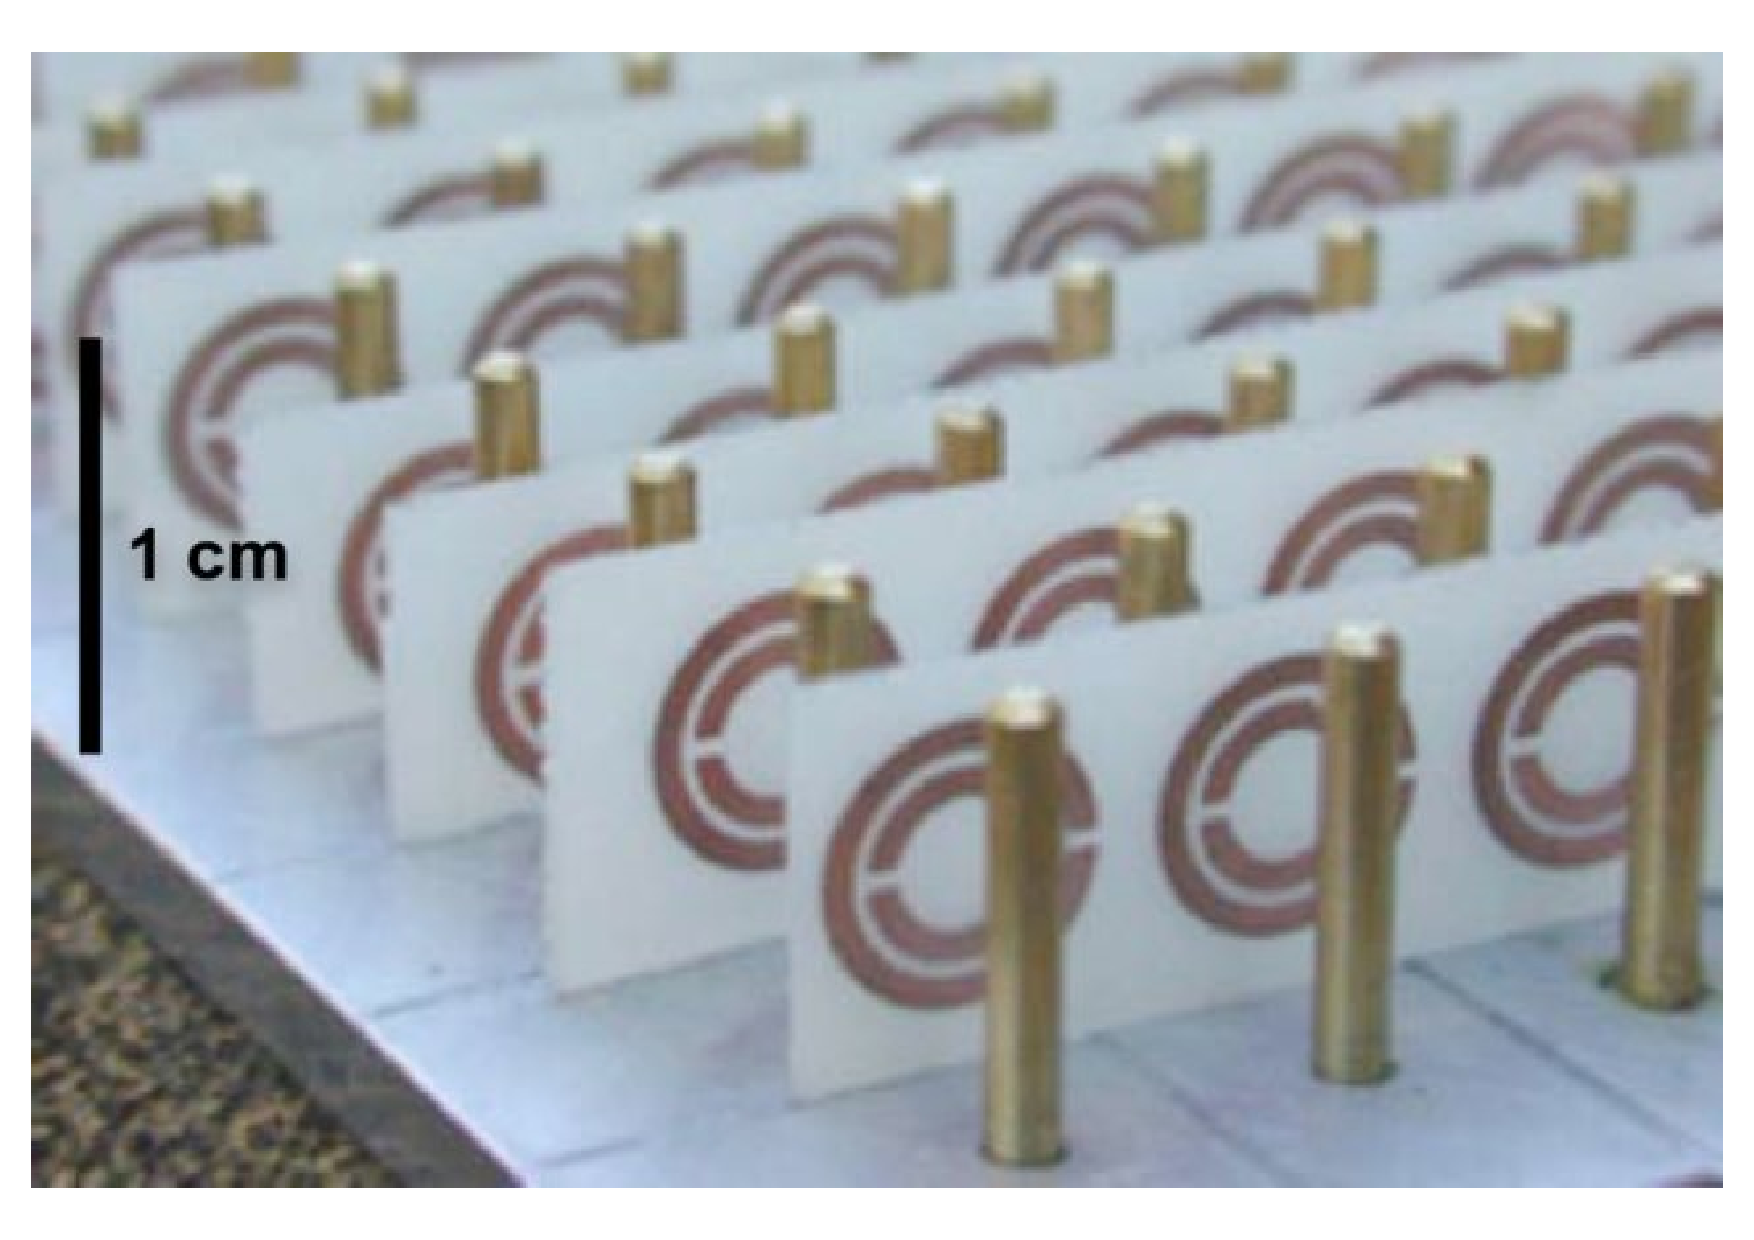
\includegraphics[width=\textwidth]{Figures/Negative_index.pdf}
            \caption{Negative refractive index metamaterial for microwaves. \cite{Ung}}
            \label{fig:Negative_index}
        \end{figure}
        \vspace{-8mm}
        \begin{figure}
            \centering
            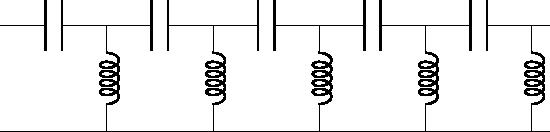
\includegraphics[width=\textwidth]{Figures/LHMM.pdf}
            \caption{Equivalent transmission line of negative index.}
            \label{fig:TL_LHMM}
        \end{figure}
        
    \end{columns}   
\end{frame}